% Scalar instruction entry source: tools/generate_scalar_instruction_catalog.py.
\subsection{\texttt{SRLI}}
\label{sec:scalar-srli}
\index{SRLI@\texttt{SRLI}}
\begin{sloppypar}\noindent\textbf{Purpose.} Logical right shift (immediate).\end{sloppypar}\smallskip
\noindent\textbf{Syntax.}\par
\begin{lstlisting}[style=ptoscalarcode]
srli SrcL, shamt, ->RegDst
\end{lstlisting}
\noindent\textbf{Encoding.}\par
\noindent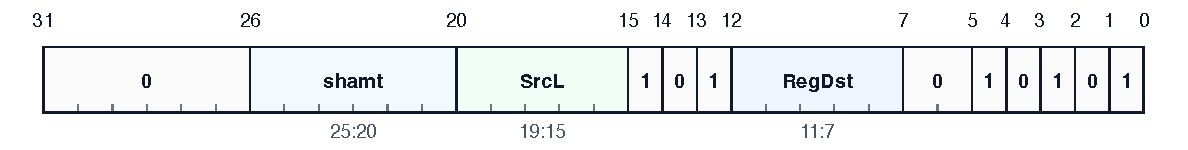
\includegraphics[width=\textwidth]{figs/encoding/scalar_instruction_entries/enc_srli.pdf}\par\smallskip
\begin{description}[leftmargin=0.18\linewidth,style=nextline]
\item[Format] \texttt{L32} \texttt{32-bit} scalar word.
\item[Pattern] \texttt{000000...........101.....0010101}.
\end{description}
\noindent\textbf{Classification.}\par
\begin{description}[leftmargin=0.18\linewidth,style=nextline]
\item[Category] Integer ALU and Bit-Manipulation.
\item[Family] Arithmetic Operation 64bit.
\item[Execution class] \texttt{ALU}; uop\_kind=ALU.
\end{description}
\noindent\textbf{Operand fields.}\par
\begin{description}[leftmargin=0.18\linewidth,style=nextline]
\item[\texttt{RegDst}] Bits \texttt{11:7 (5b)}. 5-bit scalar destination register written by this instruction; X0 is hardwired to zero, so writes to X0 are ignored.
\item[\texttt{SrcL}] Bits \texttt{19:15 (5b)}. 5-bit scalar source register used as the left input operand.
\item[\texttt{shamt}] Bits \texttt{25:20 (6b)}. 6-bit shift amount applied to the modified right operand before the ALU or address calculation uses it.
\end{description}
\noindent\textbf{Operation.}\par
\begin{lstlisting}[style=ptoscalarcode]
a = Read(SrcL)
sh = shamt
result = a >> sh
Write(RegDst, result)
\end{lstlisting}
\Needspace{0.08\textheight}
